\documentclass[10pt,a4paper]{article}
\usepackage[margin=2cm]{geometry}
\usepackage[T1]{fontenc}
\usepackage{lmodern}
\usepackage{graphicx}
\usepackage{booktabs}
\usepackage{amsmath}
\usepackage{xcolor}
\usepackage[numbers,sort&compress]{natbib}
\usepackage[hidelinks]{hyperref}
\graphicspath{{../results/figures/}}

% \writehere{...}: what each section still needs. Delete each note when the text is in.
\newcommand{\writehere}[1]{\par\noindent\fcolorbox{orange!70!black}{orange!8}{\parbox{\dimexpr\linewidth-2\fboxsep-2\fboxrule}{\small\textbf{To write:} #1}}\par}

\title{Does the G1 Obstacle Policy See the Obstacle?\\\large An Explainability Case Study of a Vision-Based PPO Policy}
\author{Javier Escobar Serrano}
\date{Explainable AI, MSc in Advanced AI, ICAI --- December 2026}

\begin{document}
\maketitle

% Length: 5-6 pages recommended, 8 maximum.

\section{Introduction}
\writehere{Problem: a PPO policy~\cite{schulman2017ppo} steers a Unitree G1 around boxes from a 64$\times$64 camera, on top of a frozen walking policy. Motivation and stakeholder: the person who decides the sim-to-real step needs to know whether the network avoids obstacles or a shortcut. State the research questions. ($\approx$0.5 page)}

\section{Data and methods}
\subsection{Environment, model and rollout dataset}
\writehere{Dataset description: origin, link, size, types, preprocessing (data/README.md has every number). Model: NatureCNN + state MLP, outputs a residual on the velocity command, clip and EMA outside the network~\cite{raffin2021sb3,todorov2012mujoco,menagerie2022}. Protocol: validation seeds, Test-ID, Test-ID-0, three OOD looks, baselines; why there is no Train-ID.}

\begin{table}[t]
\centering\small
\caption{Closed-loop evaluation, 10/20/30 boxes pooled. Rates with 95\,\% Wilson intervals; progress = distance covered / commanded.}
\label{tab:evaluation}
\resizebox{\ifdim\width>\linewidth\linewidth\else\width\fi}{!}{%
\begin{tabular}{lrllrr}
\toprule
Set & $n$ & Success \% & Box hit \% & Fall \% & Progress \\
\midrule
Validation (seeds 1000+) & 60 & 95 [86, 98] & 5 [2, 14] & 0 & 1.10 \\
Test-ID (new layouts) & 300 & 94 [90, 96] & 5 [3, 8] & 1 & 0.95 \\
OOD: blue boxes & 300 & 62 [56, 67] & 36 [31, 42] & 2 & 0.78 \\
OOD: floor tint & 300 & 71 [65, 76] & 8 [6, 12] & 0 & 0.63 \\
OOD: lighting & 300 & 93 [89, 95] & 7 [5, 10] & 0 & 1.02 \\
Baseline: walker only & 51 & 20 [11, 32] & 80 [68, 89] & 0 & 0.41 \\
Baseline: black image & 51 & 0 [0, 7] & 25 [16, 39] & 0 & 0.04 \\
Baseline: noise image & 51 & 22 [12, 35] & 78 [65, 88] & 0 & 0.44 \\
Behaviour: hide Grad-CAM region & 51 & 75 [61, 84] & 25 [16, 39] & 0 & 0.86 \\
Behaviour: hide random region & 51 & 94 [84, 98] & 6 [2, 16] & 0 & 0.94 \\
\bottomrule
\end{tabular}}
\end{table}


\subsection{Explanation methods}
\writehere{Outputs explained (raw $\mu_{vx}$, $\mu_{vy}$, $V$; orientation $s=-\mu$). Global: group permutation importance and IG aggregated by input group. Local: Grad-CAM~\cite{selvaraju2017gradcam} (conv3, conv2), Integrated Gradients~\cite{sundararajan2017axiomatic} (black and blur baselines), occlusion; Captum~\cite{kokhlikyan2020captum}. Localisation q\textsubscript{RRA}~\cite{arras2020clevrxai}. Sanity checks: randomisation~\cite{adebayo2018sanity}, ROAD~\cite{rong2022road}, agreement, q\textsubscript{LLE}/q\textsubscript{AS}~\cite{alvarezmelis2018robustness,yeh2019infidelity}, behaviour test. ($\approx$1.5 pages with 2.1)}

\section{Results}
\begin{figure}[t]
  \centering
  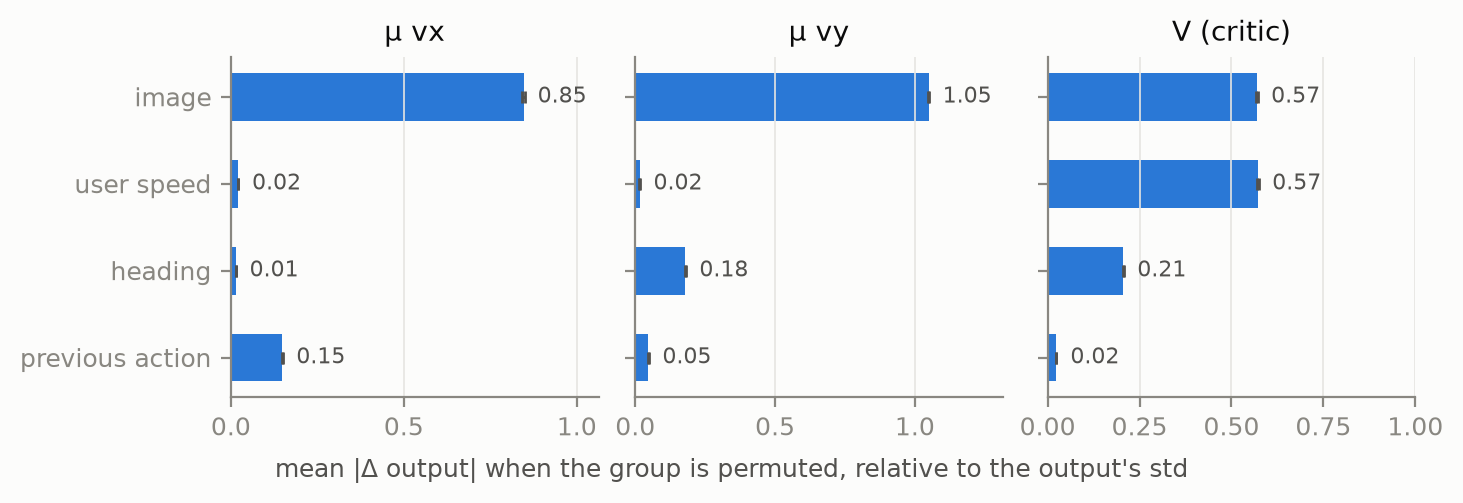
\includegraphics[width=\linewidth]{group_pfi.png}
  \caption{Group permutation importance on in-distribution frames: mean output change when one input group is taken from another episode, relative to the output's standard deviation (95\,\% intervals over 10 permutations).}
  \label{fig:pfi}
\end{figure}

\begin{figure}[t]
  \centering
  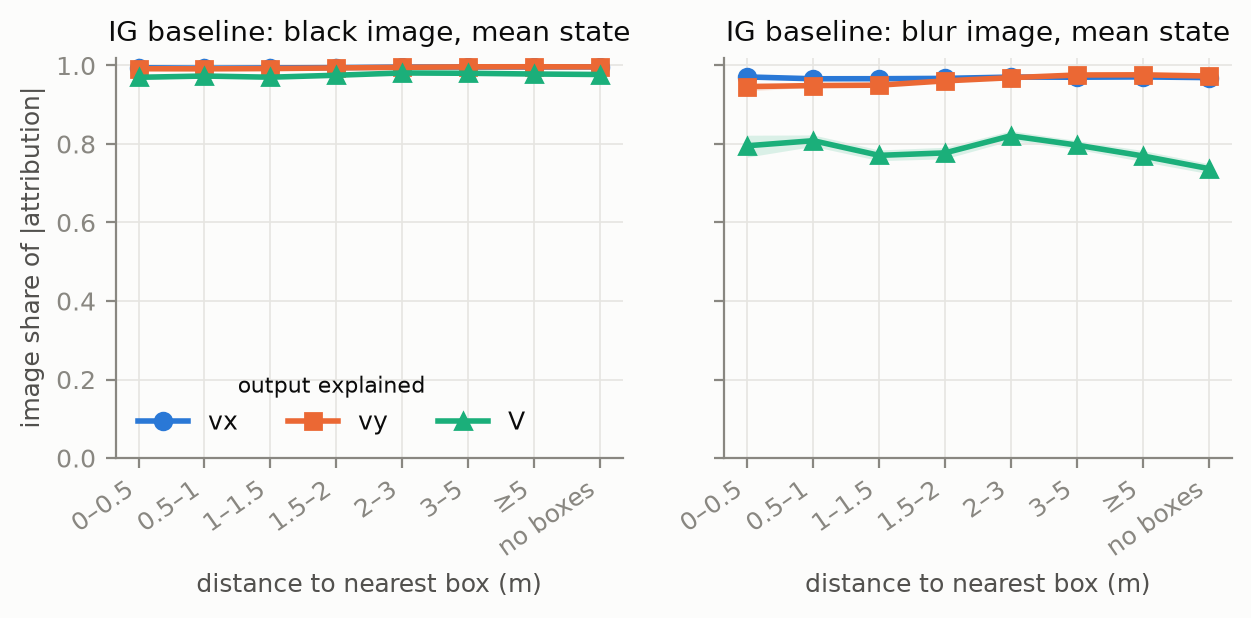
\includegraphics[width=\linewidth]{ig_image_share.png}
  \caption{Share of the absolute Integrated Gradients attribution that goes to the image, by distance to the nearest box, for two image baselines (state baseline: mean logged state, 256 steps).}
  \label{fig:ig}
\end{figure}

\begin{figure}[t]
  \centering
  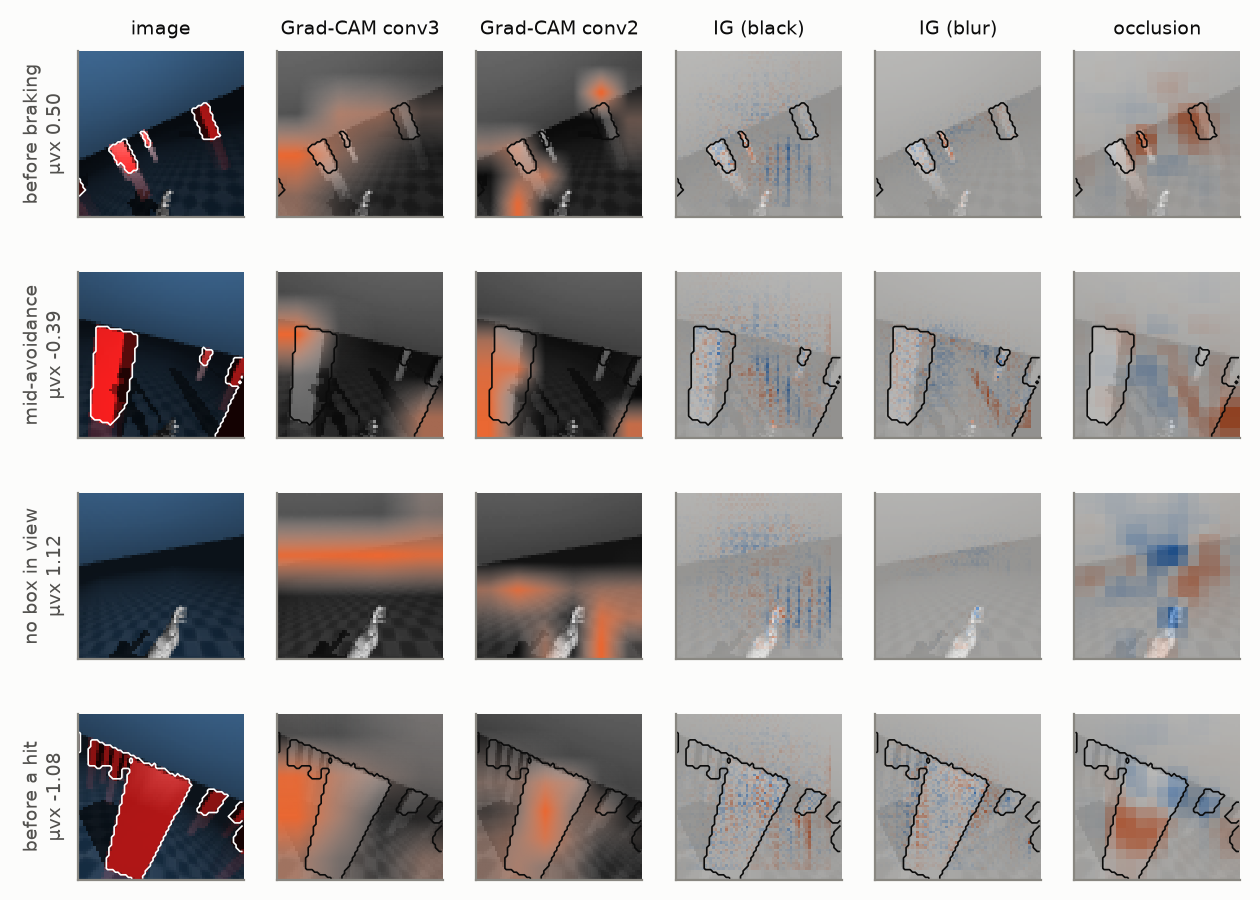
\includegraphics[width=\linewidth]{local_maps_vx.png}
  \caption{Local maps for $s=-\mu_{vx}$ (evidence for braking) on automatically selected frames. Positive evidence in orange; box outlines from the logged segmentation.}
  \label{fig:local}
\end{figure}

\begin{table}[t]
\centering\small
\caption{Localisation: q\textsubscript{RRA} divided by the random-map reference $|s|/d$ ($-\mu_{vx}$, 500 frames per set). 1 = chance.}
\label{tab:qrra}
\resizebox{\ifdim\width>\linewidth\linewidth\else\width\fi}{!}{%
\begin{tabular}{lrrrr}
\toprule
Method & Test-ID & Blue boxes & Floor tint & Lighting \\
\midrule
Grad-CAM conv3 & 3.47 & 2.53 & 3.26 & 3.16 \\
Grad-CAM conv2 & 3.08 & 3.13 & 3.44 & 2.66 \\
IG (black) & 2.29 & 2.38 & 2.36 & 2.60 \\
IG (blur) & 3.55 & 2.69 & 3.54 & 3.91 \\
Occlusion & 3.20 & 2.34 & 2.67 & 3.99 \\
\bottomrule
\end{tabular}}
\end{table}


\writehere{Evaluation metrics and what they say about generalisation (Table~\ref{tab:evaluation}). Global findings (Figures~\ref{fig:pfi}, \ref{fig:ig}). Local maps and localisation (Figure~\ref{fig:local}, Table~\ref{tab:qrra}), including one success and one failure case. ($\approx$1.5 pages)}

\section{Actions and insights}
\begin{figure}[t]
  \centering
  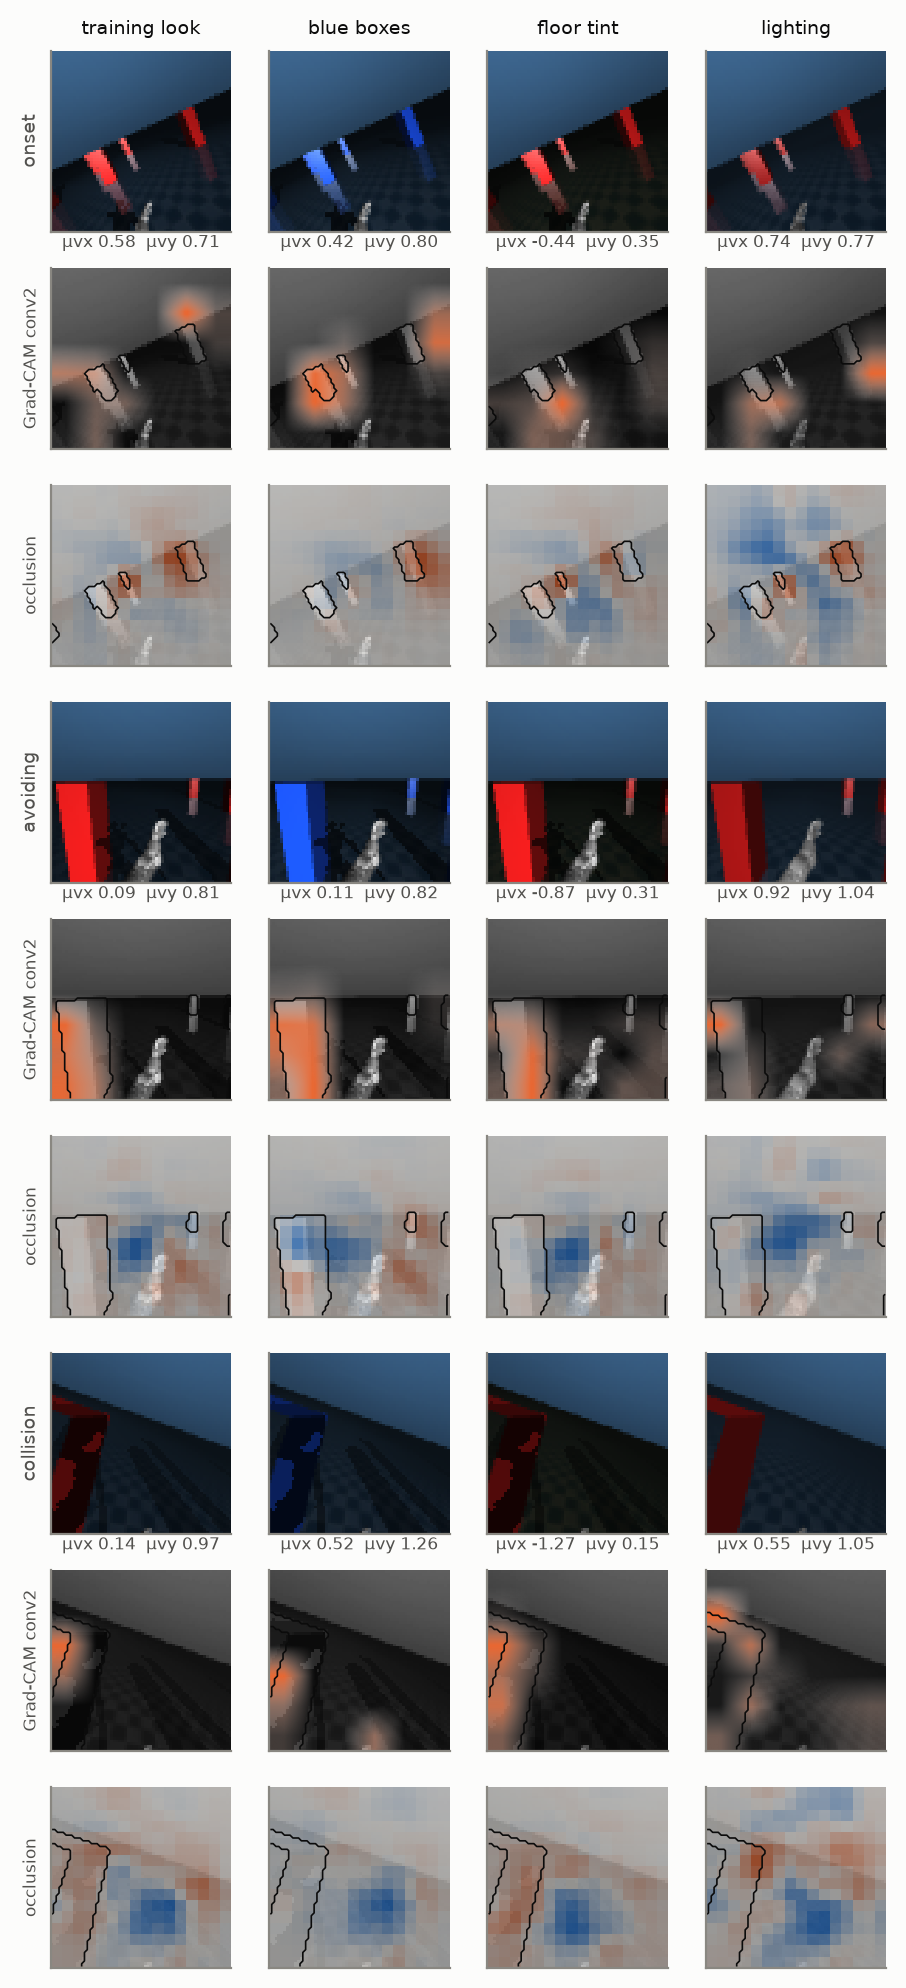
\includegraphics[width=0.62\linewidth]{pairs_vx.png}
  \caption{Logged Test-ID states re-rendered under the training look and each OOD look, with the policy's outputs and Grad-CAM (conv2) and occlusion maps for braking.}
  \label{fig:pairs}
\end{figure}

\begin{table}[t]
\centering\small
\caption{Before/after on the same seeds (paired). q\textsubscript{RRA} for Grad-CAM conv2 on $-\mu_{vx}$, divided by its random reference.}
\label{tab:before-after}
\resizebox{\ifdim\width>\linewidth\linewidth\else\width\fi}{!}{%
\begin{tabular}{llrlrlrr}
\toprule
Condition & Policy & $n$ & Success \% & Hit \% & $\Delta$ success (pp) & McNemar $p$ & q\textsubscript{RRA}/chance \\
\midrule
Test-ID & original & 300 & 94 [90, 96] & 5 &  &  & 3.1 \\
Test-ID & intervention: recolour to red & 51 & 98 [90, 100] & 2 & +0 [+0, +0] & 1.00 &  \\
Test-ID & intervention: floor colour normalisation & 51 & 98 [90, 100] & 2 & +0 [+0, +0] & 1.00 &  \\
Test-ID & fine-tune & 300 & 84 [79, 88] & 7 & -10 [-14, -6] & 5e-06 & 4.1 \\
blue boxes & original & 300 & 62 [56, 67] & 36 &  &  & 3.1 \\
blue boxes & intervention: recolour to red & 300 & 93 [90, 96] & 5 & +32 [+26, +37] & 1e-25 & 2.9 \\
blue boxes & fine-tune & 300 & 50 [45, 56] & 49 & -11 [-18, -5] & 0.001 & 1.8 \\
floor tint & original & 300 & 71 [65, 76] & 8 &  &  & 3.4 \\
floor tint & intervention: floor colour normalisation & 300 & 92 [89, 95] & 5 & +22 [+17, +27] & 2e-16 & 3.1 \\
floor tint & fine-tune & 300 & 0 [0, 1] & 41 & -71 [-76, -65] & 3e-64 & 0.1 \\
lighting & original & 300 & 93 [89, 95] & 7 &  &  & 2.7 \\
lighting & fine-tune & 300 & 93 [89, 95] & 5 & +0 [-4, +4] & 1.00 & 4.5 \\
\bottomrule
\end{tabular}}
\end{table}


\writehere{Diagnosis from the paired re-renders (Figure~\ref{fig:pairs}); the two test-time interventions and what they prove causally; the fine-tune result (Table~\ref{tab:before-after}); recommendation for the stakeholder. ($\approx$1 page)}

\section{Discussion}
\begin{table}[t]
\centering\small
\caption{Sanity checks ($v_x$ unless stated). ROAD: AUC of $|\Delta s|/\mathrm{std}(s)$, higher = more faithful. Rand.\ $\rho$: Spearman with the original map after randomising the whole network. Last two: relative map change under noise/brightness and under 1-px shifts.}
\label{tab:sanity}
\resizebox{\ifdim\width>\linewidth\linewidth\else\width\fi}{!}{%
\begin{tabular}{lrrrrrrr}
\toprule
Method & ROAD $v_x$ & ROAD $v_y$ & Rand.\ $\rho$ & q\textsubscript{LLE} & q\textsubscript{AS} & Noise \% & 1-px \% \\
\midrule
Grad-CAM conv3 & 0.206 & 0.217 & 0.19 & 0.588 & 0.0031 & 12 & 56 \\
Grad-CAM conv2 & 0.205 & 0.213 & 0.36 & 0.254 & 0.0014 & 23 & 92 \\
IG (black) & 0.092 & 0.131 & 0.45 & 0.0474 & 0.00046 & 6 & 117 \\
IG (blur) & 0.326 & 0.364 & 0.72 & 0.0174 & 0.00025 & 8 & 112 \\
Occlusion & 0.365 & 0.368 & 0.25 & 0.399 & 0.0065 & 6 & 44 \\
Random order & 0.018 & 0.021 &  &  &  &  &  \\
\bottomrule
\end{tabular}}
\end{table}


\writehere{Sanity checks (Table~\ref{tab:sanity}) and what they imply for trusting each method; faithfulness vs plausibility~\cite{jain2019attention,jacovi2020faithfulness}; IG baseline sensitivity; contrastive vs non-contrastive references; attribution on a high-level action in a hierarchical controller; temporal credit; OOD ablations vs permutation; how a stakeholder could over-trust a heatmap; sim-to-real gap; limitations and future work. ($\approx$1--1.5 pages)}

\clearpage   % place every pending figure and table before the references
\bibliographystyle{plainnat}
\bibliography{references}
\end{document}
